\documentclass[../main.tex]{subfiles}
\graphicspath{{\subfix{../images/}}}
\begin{document}

  % Precisamos agrupar melhor esses testes, dar uma logica e introduzir
  As primeiras inferências se deram quanto aos resultados da cinemática inversa. Foi observado que o sistema é capaz não só de realizar a cinemática de cada uma das pernas individualmente, como também do seu corpo em todos os 6 graus de liberdade (translações em $x, y, z$ e rotações em $roll, pitch, yaw$). A figura \ref{fig:moving_body} ilustra o movimento do corpo do robô em cada um desses graus de liberdade.

  \begin{figure}[h]
    \centering
    \caption{Titulo da Figura}
    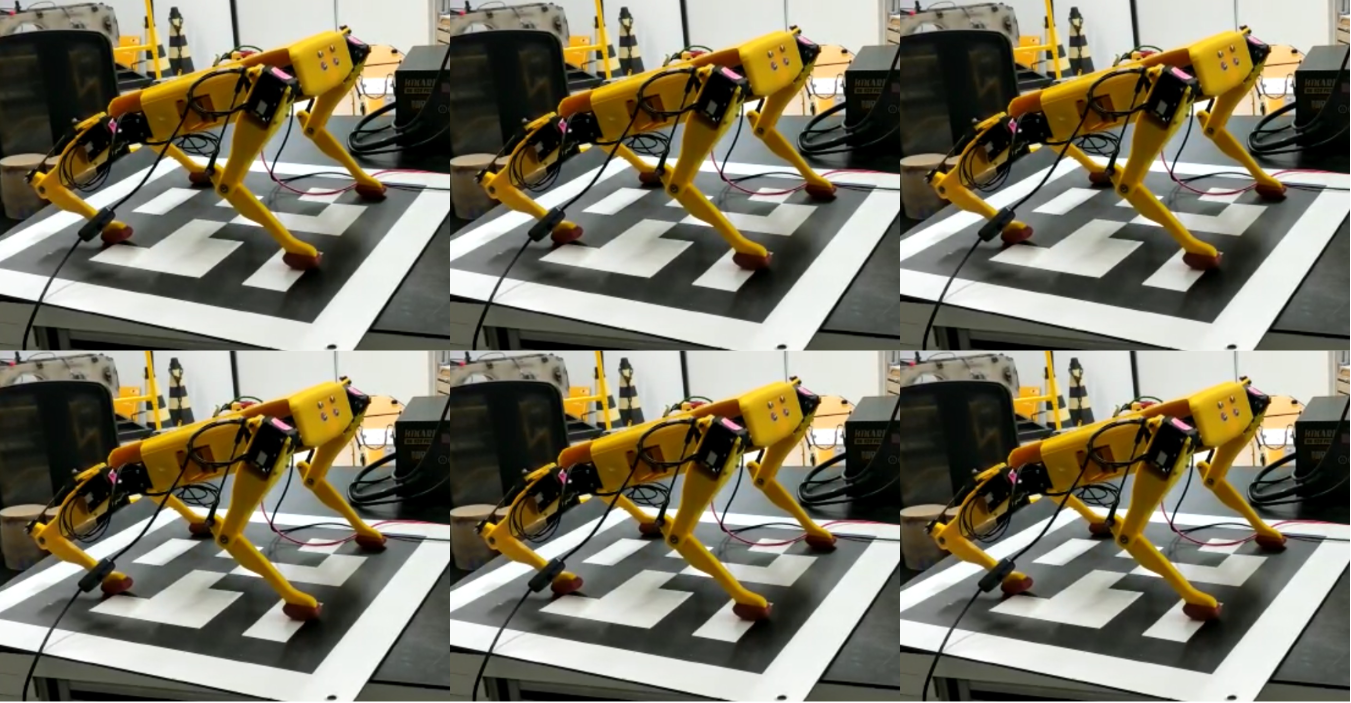
\includegraphics[width=0.48\textwidth]{moving_body.png}
    
    Fonte: XXX
    \label{fig:moving_body}
  \end{figure}

  Do mesmo modo, os gráficos da figura \ref{fig:grafico_controlling} ilustram o comportamento do sistema à variação dos \textit{setpoints} de orientação em $X$ (gráfico superior) e em $Y$ (gráfico inferior) para o corpo do robô, a partir da aplicação de diversos degraus (em azul). Nota-se que o protótipo é capaz de se adaptar rapidamente aos novos valores desejados de orientação, simultaneamente em ambos os eixos.

  \begin{figure}[h]
    \centering
    \caption{Titulo da Figura}
    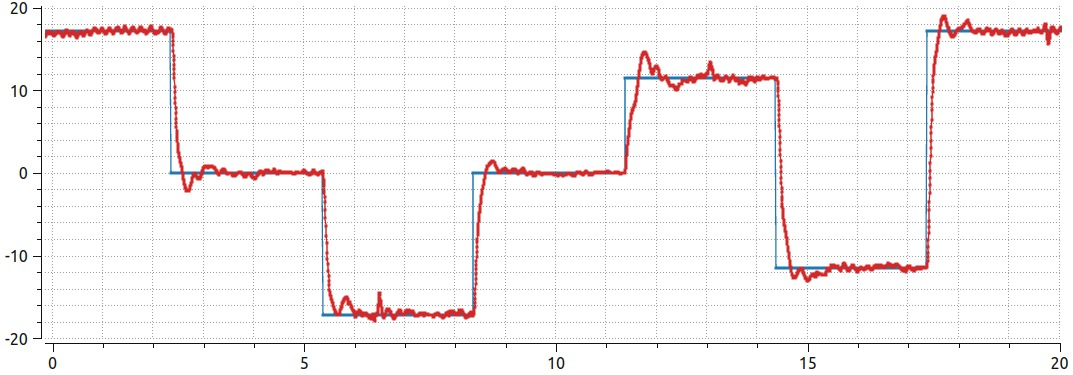
\includegraphics[width=0.48\textwidth]{grafico_controlling_X.png}
    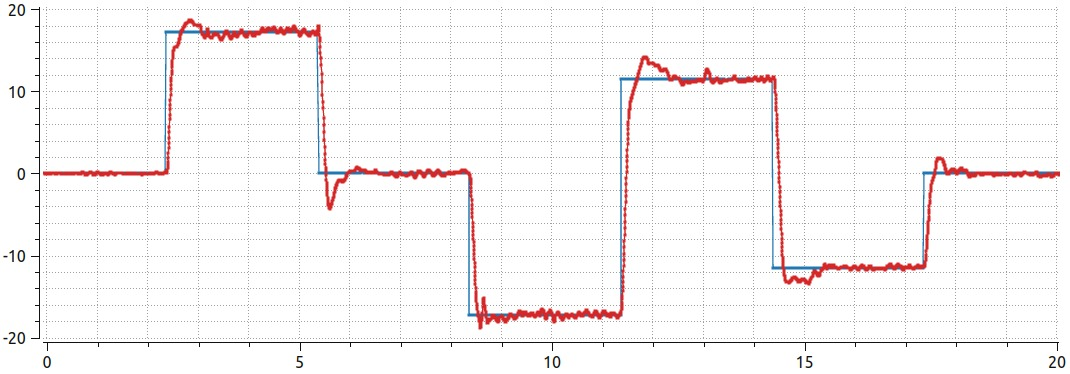
\includegraphics[width=0.48\textwidth]{grafico_controlling_Y.png}
    
    Fonte: XXX
    \label{fig:grafico_controlling}
  \end{figure}

  \subsection{Experimentos}
  Em seguida, serão apresentados os resultados dos experimentos executados diante às especificações apresentadas na metodologia.

  \subsubsection{Análise de trajetória}
  Durante este experimento, o objetivo é analisar o tempo real de execução da trajetória, as coordenadas finais $(x_f, y_f)$ da pata e a altura máxima $z_{max}$ atingida durante o passo, comparando-os com os valores desejados para cada um desses parâmetros. A tabela \ref{tab:trajetoria} traz as médias encontradas para cada um desses parâmetros durante a realização dos testes.

  \begin{table}[h]
    \caption{Titulo da Tabela}
    \centering
      \begin{tabular}{lllll}
             & $tempo (s)$ & $x_{final}(m)$ & $y_{final}(m)$ & $z_{max}(m)$ \\
      Exp. 1 & 0.559457 & 0.050349 & 0.029247 & 0.047585 \\
      Exp. 2 & 0.556770 & 0.030240 & 0.049132 & 0.046562      
      \end{tabular}

    Fonte: Autoria própria
    \label{tab:trajetoria}
  \end{table}

  Inicialmente, foram realizados dois testes de T Student para amostras independentes, o primeiro relacionando o tempo de execução da trajetória nos experimentos 1 e 2, e o segundo relacionando a altura máxima alcançada, com o intuito de verificar se os resultados se alteram para diferentes valores $(x, y)$ desejados. O resultado da análise de T Student traz um $t$ de aproximadamente $1.087$, em se tratando de tempo, e de $1.0658$ para a altura máxima alcançada durante o passo. Para uma confiabilidade de $95\%$ e um total de 58 graus de liberdade, o valor crítico $t_c$ encontrado é de $2.00$. Como ambos os valores encontrados estão dentro do intervalo de confiança ($-t_c < t < t_c$), isso mostra que não há uma diferença significativa entre as médias em cada experimento, o que significa que diferentes comandos de trajetórias em $(x, y)$ não interferem nos resultados de tempo e altura máxima do passo.
  
  Os gráficos da figura \ref{fig:grafico_trajetoria_xyz} representam um dos testes realizados para o primeiro caso ($x=0.05m$, $y=0.03m$), sendo os gráficos superiores esquerdo e direito correspondentes à trajetória em $x$ e $y$ respectivamente, e o gráfico inferior correspondente à trajetória em $z$ (altura do passo). Nota-se que, como esperado pela análise da tabela \ref{tab:trajetoria}, há um atraso na execução da trajetória (neste caso específico de aproximadamente $54ms$) e a altura máxima alcançada é levemente inferior à desejada (alcançando neste caso um valor próximo a $0.0476m$).

  \begin{figure}[h]
    \centering
    \caption{Titulo da Figura}
    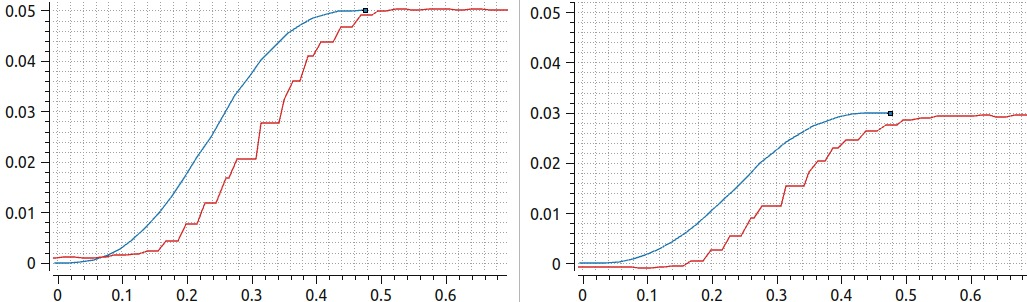
\includegraphics[width=0.48\textwidth]{grafico_trajetoria_xy.png}
    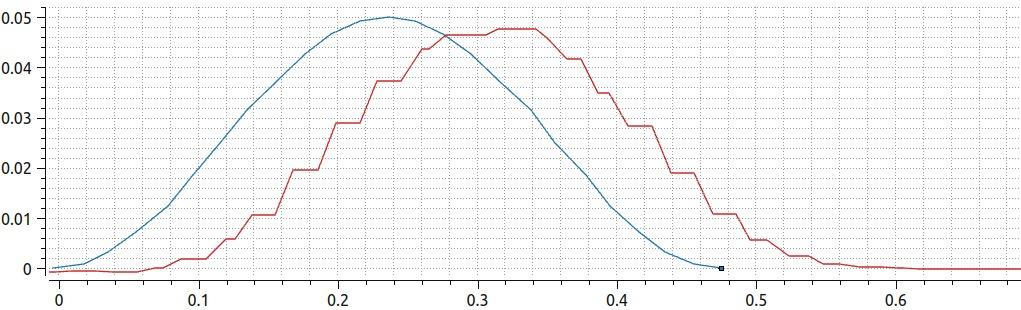
\includegraphics[width=0.48\textwidth]{grafico_trajetoria_z.png}
    
    Fonte: XXX
    \label{fig:grafico_trajetoria_xyz}
  \end{figure}

  \subsubsection{Controle de velocidade}
  Durante os testes de controle de velocidade, de maneira geral, foi observado uma caminhada eficiente em ambos os terrenos, porém, mais linear e com menor trepidação em terrenos regulares do que em terrenos irregulares. Por meio dos dados coletados, foram extraídas as informações, velocidade média da caminhada, oscilação máxima de rotação do corpo em roll e pitch e os respectivos desvios padões, apresentados na Tabela \ref{tab:vel_stab}. Assim, foi observado que a menor oscilação em roll e em pitch ocorreu no terreno regular utilizando o controle de rotação, enquanto que a maior oscilação ocorreu nas condições opostas (teste 3).  Por outro lado, o robô se aproximou mais vezes da velocidade solicitada no terreno regular combinado ao controle de rotação, enquanto que no irregular com controle de rotação foi apresentada uma velocidade média inferior e baixa consistência nos dados.

  \begin{table}[]
    \caption{Titulo da Figura}
    \centering
    \begin{tabular}{ccccc}
      \hline
      & 1 & 2 & 3 & 4 \\ \hline
      Terreno & Reg. & Reg. & Irreg. & Irreg. \\ \hline
      \begin{tabular}[c]{@{}c@{}}C. R.\end{tabular} & Não & Sim & Não & Sim \\ \hline
      \begin{tabular}[c]{@{}c@{}}Vel. \\ (m/s) \end{tabular} &   0.0292   &  0.0333  &   0.0297   & 0.0277  \\ \hline
      \begin{tabular}[c]{@{}c@{}} $\sigma_{Vel}$  \\ (m/s) \end{tabular} & 0.00135 & 0.00079 & 0.00197 & 0.00241 \\ \hline
      \begin{tabular}[c]{@{}c@{}} $\Delta_{Roll}$ \end{tabular} & 12.541\degree & 8.742\degree & 13.897\degree & 12.168\degree \\\hline
      \begin{tabular}[c]{@{}c@{}} $\sigma_{Roll}$ \end{tabular}  & 2.416\degree & 2.145\degree & 1.802\degree & 3.270\degree \\ \hline
      \begin{tabular}[c]{@{}c@{}} $\Delta_{Pitch}$ \end{tabular} & 11.458\degree & 8.295\degree & 15.189\degree & 13.182\degree \\ \hline
      \begin{tabular}[c]{@{}c@{}} $\sigma_{Pitch}$ \end{tabular}  & 1.826\degree & 2.386\degree & 1.441\degree & 2.944\degree \\ \hline

    \end{tabular}
    Fonte: Autoria própria
    \label{tab:vel_stab}
  \end{table}

  A fim de avaliar se o controle de rotação aqui proposto contribuiu de fato na estabilidade da caminhada, utilizaremos o teste T-Student para amostras independentes, com um nível de confiança de 95\%. Então, foi proposto como hipotése nula que o uso do controle de rotação do corpo não contribui na oscilação de rotação do corpo. Dessa forma, a análise foi feita entre os testes 1 e 2, e entre os testes 3 e 4, ou seja, considerando o mesmo terreno. O resultado desta análise nos mostrou que para terrenos planos a hipotése nula pode ser rejeitada, pois o p-valor se mostrou menor que 0,05 (0,00033) . Entretanto, para terrenos irregulares não houve mudanças significativas na estabilidade do protótipo, dado p-valor 0,0778, nos levando a considerar a ocorrência de causalidades no teste. 
    
  \subsubsection{Plano inclinado}
  Durante este experimento, contatou-se que o robô possui a habilidade de andar por terrenos com 5,336\degree de inclinação, figura \ref{fig:tests3-4}. 

  \subsubsection{Superação de obstáculos}
  O último experimento, constatou que o robô é capaz de ultrapassar obstáculos de até 5cm de altura. Para isso foram testados três degraus de 2, 4 e 5 cm de altura, sendo os dois últimos apresentados na figura \ref{fig:tests3-4}.

  \begin{figure}[h]
    \centering
    \caption{Titulo da Figura}
    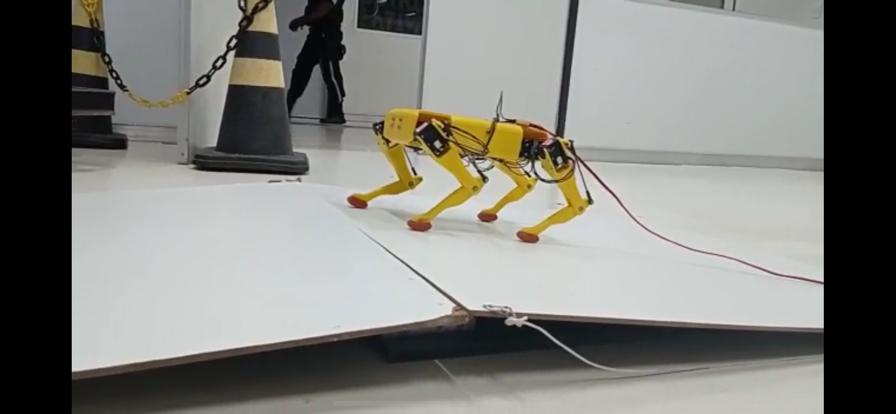
\includegraphics[width=0.48\textwidth]{ramp_test.jpeg}
    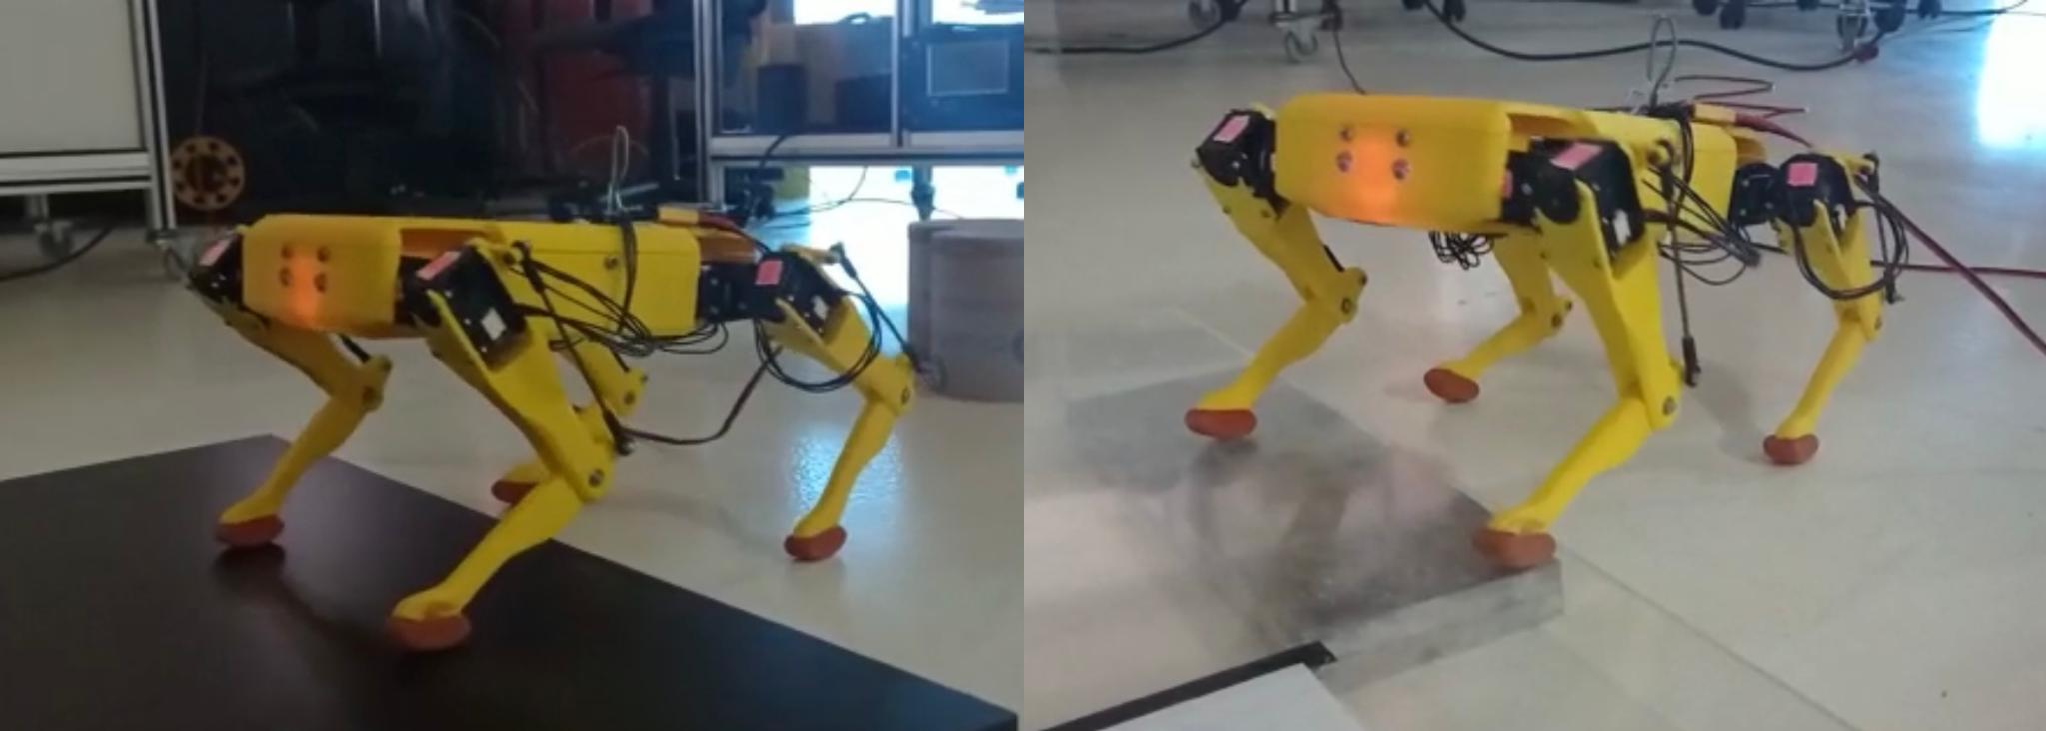
\includegraphics[width=0.48\textwidth]{test4.png}

    Fonte: XXX
    \label{fig:tests3-4}
  \end{figure}

   


\end{document}